\chapter{多元函数微分学}

\section{导数与微分}

\subsection{基本定义}

\begin{definition}{方向导数, 偏导数}
    设开集$E \subseteq \R ^n$, 函数$f:E \to \R$, $x_0 \in E , v \in \R ^n$. 定义$f$在$x_0$处\textit{沿$v$的方向导数}为下列极限(如果存在): $$\frac{\p f}{\p v}(x_0) := \lim_{h \to 0} \frac{f(x_0+hv)-f(x_0)}{h}.$$
    特别地, 令$e_i$为第$i$个坐标为$1$, 其余为$0$的单位向量, 则称沿$e_i$的方向导数为该方向上的\textit{偏导数}. 
\end{definition}

偏导数是容易求得的: 由于$h$不影响$e_i$方向以外的方向, 只需将整个函数视作关于$e_i$的一元函数求导即可. 

稍后会验证(实际上是显然的), 当$f$可微时成立$\frac{\p f}{\p v_1}(x_0) + \frac{\p f}{\p v_2}(x_0) = \frac{\p f}{\p (v_1+v_2)}(x_0)$. 此时只需计算$f$的所有偏导数即可得到任意方向导数. 反过来, 当$f$不可微时, 即使偏导数均存在, 也不能保证方向导数存在(更不用说如此计算了). 

\begin{example}
	考虑$f(x,y)=\begin{cases}
		\frac{xy}{x^2+y^2} & (x,y) \neq (0,0) \\ 0 & (x,y)=(0,0)
	\end{cases}$. 则$f$的两个偏导数在$(0,0)$均为$0$, 但是$\frac{\p f}{\p v} = \lim_{h \to 0} \frac{v^1v^2}{h((v^1)^2+(v^2)^2)}$不存在, 其中$v_1v_2 \neq 0$. 
\end{example}

方向导数有清晰的几何意义: 设曲线$\gamma :(-\delta,\delta) \to \R ^n$是$C^1$的. 我们有$$\frac{\dif}{\dif t} \big|_{t=0} (f|_{\rge \gamma} \circ \gamma) = \frac{\p f}{\p \gamma '(0)} (\gamma (0)). $$
这一式子不难验证. 在图像上(这里我们以$\R ^2$模拟$\R ^n$, 并将$\R$置于$\R ^n$的法向量方向上), 这一式子大概在说: 在$\gamma '(0)$方向上求导, 相当于考虑$f$在$\gamma$这一条曲线之上的部分(实际上是$\R \to \R$的, 但在图像上看起来像是曲线), 再在这部分上求$0$处的导数. 换句话说, 针对一个方向$v$, 我们只需考虑顺着该方向上$f$的行为即可. 

\begin{figure}[H]
	\centering
	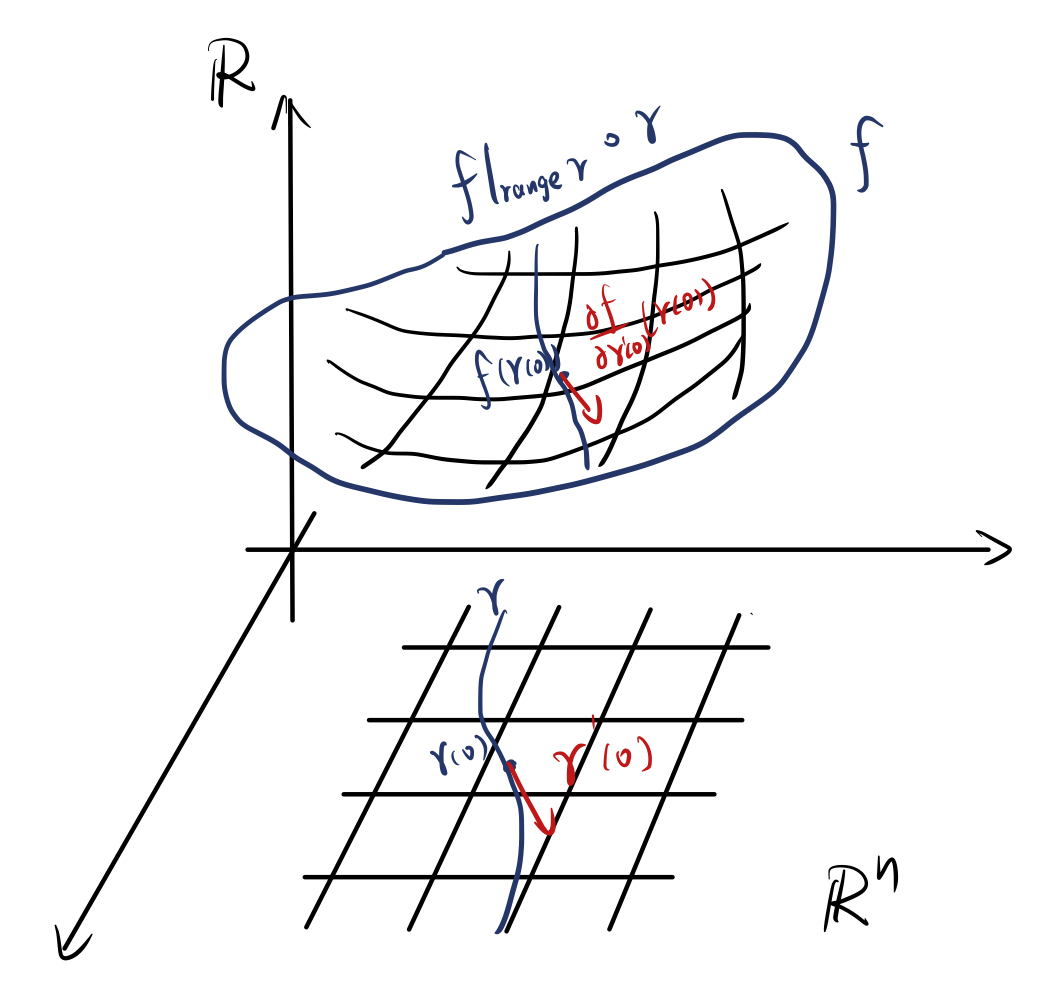
\includegraphics[width=7cm]{attachment/IMG_3923.jpg}
	\caption{方向导数的几何意义}
\end{figure}

这里需要就多元函数的图像一事做些补充. 

首先, 若是从函数角度来看, 此处的$\R ^n \times \R$就是$(x_0,f(x_0))$所生活的空间\footnote{这部分内容不会严格区分$\R ^n \times \R ^m$与$\R ^{n+m}$. }, $f$在这里形成了图像$\Gamma _f$. 容易感知到, 两个字空间$\R$与$\R ^n$“天生”地不相干, 或者说这种描述严重依赖于坐标系的选取. 然而, 正如我们乐于将$\R \times \R = \R ^2$视作一个正常的平面, 这里的$\R ^n \times \R$也可视作一整个空间, 即任意一个$\R$上的$n+1$维向量空间, 这就不依赖坐标系了. 如果的确需要在这一空间中描述某个形状, 此时应当使用(某个坐标系下的)隐函数$f(x_0^1,\cdots ,x_0^n,x_0^{n+1})=0$. 也就是在这两种描述中互相转化: $$\{ (x,f(x)) \in \R ^n \times \R : x \in \R \} = \{ (x,y) \in \R ^n \times \R : F(x,y)=0,F(x,y)=(0,y-f(x)) \}.$$
作为例子, $\R ^3$中的单位球面$S^2$可表示为$2$个函数图像$f_+(\R ^2),f_-(\R ^2)$的并(其中$f_{\pm} (x,y)= \pm \sqrt{1-x^2-y^2}$), 亦可表示为$f^{-1}(\{ 0 \})$(其中$f(x,y,z) = x^2+y^2+z^2-1$). 大多数时候后者的形式更加简洁且易于推广; 并且我们很快就会看到, 利用$f^{-1}(S)$的形式更容易判断该形状是否是光滑子流形, 并且求出其维数. 

其次, 在一元微分学部分, 我们体会到了“导数”就等于“切线斜率”的想法. 我们希望在多元微分学中找到对应的想法. 

将斜率放在我们强行捏造的图像上, 它表示$x$轴(定义域)上的单位距离对应$y$轴(值域)距离的值, 即两点$(x_1,f(x_1)),(x_2,f(x_2))$的斜率为$\frac{f(x_2)-f(x_1)}{x_2-x_1}$, 这里最关键的一步在于单位化. 若要将其推广至多元函数, 由于单位化的操作无法对两个向量实施, 我们不得不单独考虑一个方向上的比值, 再将这些比值按方向加总(形象地说就是将$x$轴绕$\R ^n$转一圈再将结果矢量求和). 问题在于, 加总后的结果还能反映每个方向的情况吗? 

幸好我们研究的是向量空间$\R ^n$. 线性代数告诉我们的确可以(一组基和全体向量等价). 此时不难猜测点$(x_1,f(x_1)),(x_2,f(x_2))$间的“斜率”是一个$\R ^n$的向量$k$, 且$k= \frac{f(x_2^1)-f(x_1^1)}{x_2^1-x_1^1}e_1 + \cdots + \frac{f(x_2^n)-f(x_1^n)}{x_2^n-x_1^n}e_n$. 更进一步, 当$f$存在所有偏导数时, 在某点$x_0$处的斜率就是$\frac{\p f}{\p e_1}(x_0)e_1 + \cdots + \frac{\p f}{\p e_n}(x_0)e_n$. 进而, 可以定义$f$的\textit{梯度}$\nabla f$使得$\nabla f(x_0)$是$x_0$处的斜率. 

需要注意, 这里我们用一个$\R ^n$上特定的坐标系描述$f$. 实际上更换坐标系并不会影响梯度, 这从几何图像上是显然的. 另外, 在引入切空间的概念后, 可以证明一个优美的结论: $\nabla f(x_0)$就是切空间$T_{x_0}(f^{-1}(0))$的法向量. 

回到正题, 我们来定义多元函数的微分. 

\begin{definition}{微分}
	设开集$E \subseteq \R ^n$, 函数$f: E \to \R$, $x_0 \in E$, $v \in \R ^n$. 称$f$在$x_0$处\textit{可微}, 若存在线性映射$T$使得$$f(x_0+v) = f(x_0) + T(v) + o(v),\qquad v \to 0$$
	对任意的$v$成立. 此时记$f$的\textit{微分}$\dif f$满足$\dif f(x_0)=T$. 
\end{definition}
\begin{remark}
	微分的定义并不依赖坐标系(任意赋范线性空间均可定义). 这也是多元函数的微分与导数始终存在很大差距的根本原因. 
\end{remark}

将微分的定义式写成$n$个方程, 实际上我们可以得到: 若$f$在$x_0$可微, 则$$ \frac{\p f}{\p v}(x_0) = \dif f(x_0)(v) = \sum_{i=1}^{n} \frac{\p f}{\p x_i}(x_0)v^i.$$
特别地, 此时$f$的所有方向导数均存在. 这也证明了上面提到过的式子$\frac{\p f}{\p v_1}(x_0) + \frac{\p f}{\p v_2}(x_0) = \frac{\p f}{\p (v_1+v_2)}(x_0)$. 

反过来, 我们好奇偏导数的存在性将如何影响可微性. 

\begin{proposition}{}
	设开集$E \subseteq \R ^n$, 函数$f: E \to \R$, $x_0 \in E$. 若$f$在$x_0$处的所有偏导数在$x_0$附近均存在且$\frac{\p f}{\p x_i}$均连续, 则$f$在$x_0$处可微. 
\end{proposition}
\begin{remark}
	请注意, 该命题的条件是偏导数在$x_0${\color{blue} 附近}存在. 直观上来看, 一个点处的偏导数并不能给出什么有用的信息, 但是一片区域上的偏导数能够描述函数的某种趋势. 
\end{remark}
\begin{proof}
	我们尝试证明$r(v)=f(x_0+v)-f(x_0)-\sum_{i=1}^{n} \frac{\p f}{\p x_i}(x_0)v^i$在$v \to 0$时是$o(v)$的. 计算可得: 
	\begin{align*}
		r(v) &= f(x_0^1+v^1,\cdots ,x_0^n+v^n) - f(x_0^1,\cdots ,x_0^n) - \sum_{i=1}^{n} \frac{\p f}{\p x_i}(x_0)v^i \\
		&= \sum_{i=1}^{n} \left( f(\cdots ,x_0^{i-1}+v^{i-1},{\color{blue} x_0^{i}+v^{i} },x_0^{i+1},\cdots) - f(\cdots ,x_0^{i-1}+v^{i-1},{\color{blue}x_0^{i} },x_0^{i+1},\cdots) - \frac{\p f}{\p x_i}(x_0)v^i \right) \\
		&= \sum_{i=1}^{n} \left( \frac{\p f}{\p x_i}(\xi _i)v^i - \frac{\p f}{\p x_i}(x_0)v^i \right). 
	\end{align*}
	其中, 最后一步对蓝色部分使用一元函数的Lagrange中值定理. 由Cauchy不等式可得$|r(v)| \leq |v| \cdot \sum_{i=1}^{n}\left| \frac{\p f}{\p x_i}(\xi _i) - \frac{\p f}{\p x_i}(x_0) \right|$, 这就证明了原命题. 
\end{proof}




\subsection{导数与微分的计算}

\subsection{$\R ^n$中的子流形}

\newpage
\section{中值定理与Taylor公式}

\subsection{微分中值定理}

\subsection{Taylor公式}

\subsection{多元函数的极值}

\newpage
\section{隐函数定理}

\subsection{反函数定理}

\subsection{隐函数定理}


\newpage
\section{隐函数定理的应用}

\subsection{流形版本的隐函数定理}

\subsection{Lagrange乘子法}